\documentclass[11 pt, a4paper]{article}  % list options between brackets
\usepackage[nottoc,notlof,notlot,numbib]{tocbibind}
\usepackage[margin=1.1 in]{geometry}
\usepackage{fancyhdr}
\usepackage{manfnt}
\usepackage{pgf}
\usepackage{amsmath,amssymb,natbib,graphicx}
\usepackage{amsfonts}
\DeclareMathAlphabet{\mathpzc}{OT1}{pzc}{m}{it}
\usepackage{bbm}
\usepackage{hyperref}
\usepackage{float}
\usepackage{mathrsfs} %mathscr{A}
\usepackage{subfigure}
\usepackage{chngpage}

\usepackage{times}
\usepackage{latexsym}
\usepackage{caption}

\newtheorem{axiom}{Axiom}[section]
\newtheorem{result}{Result}[section]
\newtheorem{example}{example}[section]
\newtheorem{definition}{Definition}[section]
\newtheorem{principle}{Principle}[section]
\newtheorem{theorem}{Theorem}[section]% list packages between braces

% type user-defined commands here
%\newcommand{\vmu}{{\bf \mu}}
%\newcommand{\vtheta1}{{\bf \theta^{(1)}}}
%\newcommand{\vtheta2}{{\bf \theta^{(2)}}}
%\newcommand{\vpi}{{\bf \pi}}}

\newcommand{\gm}{\gamma}

\begin{document}

\title{Summary of Short-term Research Objectives}   % type title between braces
\author{Detian Deng}         % type author(s) between braces
\date{\today}    % type date between braces
\maketitle

%\begin{abstract}
%\end{abstract}

\section{Model Specification}             % section 1
Let $L$ be a K-dimensional Bernoulli random variable denoting the true state.
Consider the general log linear model:
\begin{align*}
f(l; \Theta) = & \exp \{\Theta_1^T l + \Theta_2^{T} u_2 + \ldots + \Theta_K^T u_K - A^*(\Theta)\}
\end{align*}
where $U_k$ is a ${K \choose k} \times 1$ vector of k-way cross-products, $k = 1,\ldots,K$,  and $\Theta = (\Theta_1,\ldots, \Theta_K)$ contains the the natural parameters, which is a $(2^K-1) \times 1$ vector.\\
\ \\
Model restrictions, let $\tilde{l} = (l,u_2,\dots,u_K)^T$, and $S = \sum_{j=1}^K L_j = s$ has some fixed pmf 
\begin{align}
\pi(s) := & P(S=s)\nonumber \\ 
= & \frac{1}{A(\Theta)} \sum_{\tilde{l}:S=s}\exp \{ \Theta^T \tilde{l}\}  \text{ , } s = 0,1,\ldots, K \\
A(\Theta) = & \sum_{\tilde{l}:l\in \{0,1\}^K}\exp \{ \Theta^T \tilde{l}\}
\end{align}


\newpage
\section{Posterior Distribution}
\begin{align*}
P(\mu, \theta^{(2)} |L) \propto & P(L, \mu, \theta^{(2)}) \\
\propto &  P(L, \mu ,\theta^{(1)},\theta^{(2)},\pi) \\
\propto & P(L | \mu, \theta^{(1)},\theta^{(2)},\pi) P(\mu, \theta^{(1)},\theta^{(2)},\pi)\\
\propto & P(L | \theta^{(1)},\theta^{(2)}) P(\theta^{(1)},\theta^{(2)} |\mu, \pi ) P(\mu) P(\pi)\\
\propto & \text{QE}(L; \theta^{(1)},\theta^{(2)}) \text{UFR}(\theta^{(1)},\theta^{(2)} |\mu, \pi ) \text{N(logit(}\mu),\Sigma) \text{tPois}(\pi)
\end{align*}
where QE is the second-order log linear model.\\
UFR is a Multivariate distribution of $[\theta^{(1)},\theta^{(2)}|\mu, \pi]$ subject to non-linear constrains:\\
 $M( \theta^{(1)},\theta^{(2)}) =\mu$ and $\Pi (\theta^{(1)},\theta^{(2)}) = \pi$, which can be sampled by a two-step procedure.\\
tPois is a truncated conjugate Poisson distribution defined as:
\begin{align*}
\pi \sim & \text{Dirichilet}(\text{hist}(\vec{s}))\\
s \sim & \frac{\lambda^s}{s!}e^{-\lambda}/[1- \sum_{s>K}\frac{\lambda^s}{s!}e^{-\lambda}]
\end{align*}

\subsection{On sampling $[\Theta |\mu, \pi]$}

\subsubsection{General model}
For General model, $\tilde{L}$ is a square matrix with dimension $J_1 = 2^K-1$. Recall that 
\begin{align}
A(\Theta) = & \frac{1}{\pi(0)} \nonumber \\
\pi(s) = & \frac{1}{A(\Theta)} \sum_{\tilde{l}:S=s}\exp \{ \Theta^T \tilde{l}\}  \text{ , } s = 1,\ldots, K \\
\mu_k = & \frac{1}{A(\Theta)} \sum_{\tilde{l}:l_k=1}\exp \{ \Theta^T \tilde{l}\}  \text{ , } k = 1, \ldots, K
\end{align}
Define intermediate parameter $\phi_j = \exp(\theta^T\tilde{l}_j) >0$, $\Theta = (\theta^{(1)},\theta^{(2)}, \ldots, \theta^{(K)}), j= 1, \ldots, J_1$ and two $K \times J_1$ sub-design matrices $B$, $C$, where $B[k,j] = 1(\tilde{l}_j^T 1=k)$, $C[k,j] = 1(\tilde{L}[j,k]=1)$. Thus (6) and (7) become
\begin{align*}
\vec{\phi} > & 0\\
B \vec{\phi} = & \vec{\pi}/\pi(0)\\ 
C \vec{\phi} = & \vec{\mu}/\pi(0)
\end{align*}
Note that B and C are not independent constraints and should be compatible so that $\binom{B}{C}$ has rank $2K-1$.\\
Based on [1][2], we can sample $\vec{\phi}$ from Uniform distribution subject to the above linear constraints efficiently and robustly. Then $\Theta$ are the solutions to the linear system ($J_1$ equations with $J_1$ unknowns):
\[\tilde{L}\Theta = \log \vec{\phi}\]
Since $\vec{\phi}$ fully specifies all cell probabilities, the posterior distribution becomes 
\[ P(\mu, \vec{\phi} |L) \propto \text{LL}(L; \vec{\phi}) \text{UFR}(\vec{\phi} |\mu, \pi ) \text{N(logit(}\mu),\Sigma) \text{tPois}(\pi)\]


\subsubsection{QE model}
For QE model, $\tilde{L}$ is a $J_1\times J_2$, where $J_1 = 2^K-1, J_2 = \frac{1}{2}K(K+1)$.  Let $\theta = (\theta^{(1)},\theta^{(2)})$, we have a over-determined linear system after sampling $\vec{\phi}$: ($J_1$ equations with $J_2$ unknowns)
\[\tilde{L}\theta = \log \vec{\phi}\]
In this case, we can first find $\Theta$ as in last section and then solve the constrained Least Square problem to get the QE parameter estimates $\theta$:
\begin{align*}
\text{minimize } & ||\theta - \Theta||^2_2 \\
\text{subject to } & B e^{\tilde{L}\theta} =  \vec{\pi}/\pi(0)\\ 
\text{and } & C e^{\tilde{L}\theta} =  \vec{\mu}/\pi(0)
\end{align*} 

\newpage
\subsection{Example for $K=3$}
\subsubsection{The Feasible Space}
For $K=3$ with the General Log-linear model,
$\Theta = (\theta_1, \theta_2, \theta_3, \theta_{12}, \theta_{13}, \theta_{23}, \theta_{123})^T$\\
$\Phi = (\phi_1 = \exp{(\theta_1)}, \ldots, \phi_4 = \exp{(\theta_1 + \theta_2 + \theta_{12})}, \ldots, 
\phi_7 = \exp{(\theta_1 + \theta_2 + \theta_3 + \theta_{12} + \theta_{13} + \theta_{23} + \theta_{123})} )^T$
When we made prior assumption on $\vec{\mu} = (\mu_1, \mu_2, \mu_3)^T$ and $\pi_0$, the sampling constraints are:
\begin{align*}
\sum_{i=1}^7 \phi_i = & \frac{1-\pi_0}{\pi_0}\\
\phi_1 + \phi_4 + \phi_5 + \phi_7 = & \frac{\mu_1}{\pi_0}\\
\phi_2 + \phi_4 + \phi_6 + \phi_7 = & \frac{\mu_2}{\pi_0}\\
\phi_3 + \phi_5 + \phi_6 + \phi_7 = & \frac{\mu_3}{\pi_0}\\
\phi_i \in & (0, \frac{1}{\pi_0}-1)
\end{align*}
And an implicit assumption is $\mu_k < 1 - \pi_0 \leq \sum_{k=1}^3 \mu_k$.\\

By applying row reduction to the augmented matrix of the above $4$ equations, we have 
\begin{align*}
\begin{pmatrix}
-1 & -1 & -1 & 0  & 0 & 0 & 1 & -\frac{\sum \mu_k + 2\pi_0 -2}{\pi_0}\\ 
0 & 1 & 1 & 0 & 0 & 1 & 0 & \frac{\mu_1+\pi_0-1}{\pi_0} \\ 
1 & 0 & 1 & 0 & 1 &  & 0 &  \frac{\mu_2+ \pi_0-1}{\pi_0}\\ 
1 & 1 & 0 & 1 & 0 & 0 & 0 & \frac{\mu_3 + \pi_0-1}{\pi_0}
\end{pmatrix}
\end{align*}
Thus let $\phi_1 = u, \phi_2 = v, \phi_3 = w $, the feasible region of $\Phi$ is defined by:
\begin{align*}
\begin{pmatrix}
u\\ 
v \\ 
w\\ 
-u-v-\frac{\pi_0-1+\mu_3}{\pi_0}\\
-u-w-\frac{\pi_0-1+\mu_2}{\pi_0}\\
-v-w-\frac{\pi_0-1+\mu_1}{\pi_0}\\
u+v+w+\frac{\sum \mu_k + 2\pi_0 -2}{\pi_0}
\end{pmatrix}  = 
\begin{pmatrix}
0\\ 
0\\ 
0\\ 
-\frac{\pi_0-1+\mu_3}{\pi_0}\\
-\frac{\pi_0-1+\mu_2}{\pi_0}\\
-\frac{\pi_0-1+\mu_1}{\pi_0}\\
\frac{\sum \mu_k + 2\pi_0 -2}{\pi_0}
\end{pmatrix}  + u
\begin{pmatrix}
1\\ 
0 \\ 
0\\ 
-1\\
-1\\
0\\
1
\end{pmatrix} + v
\begin{pmatrix}
0\\ 
1 \\ 
0\\ 
-1\\
0\\
-1\\
1
\end{pmatrix}  + w
\begin{pmatrix}
0\\ 
0 \\ 
1\\ 
0\\
-1\\
-1\\
1
\end{pmatrix}  
\end{align*}
and $\phi_i \in  (0, \frac{1}{\pi_0}-1)$ for $i = 1, \ldots, 7$ (*)\\

To sample $(u,v,w)$ from its feasible space, we can do as follow:
Let $a = max\{\mu_2,\mu_3\}$, $b = max\{\mu_1,\mu_3\}$, $c = max\{\mu_1,\mu_2\}$
\begin{enumerate}
\item Sample $u$ from Unif($0$, $\frac{1-a-\pi_0}{\pi_0}$).
\item Sample $v$ from Unif($0$, $\frac{1-b-\pi_0}{\pi_0}$) .
\item Sample $w$ from Unif($0$, $\frac{1-c-\pi_0}{\pi_0}$) .
\end{enumerate}
Then reject all $(u,v,w)$ samples such that the resulted  $\phi$ does not satisfy condition (*). Also note that the Monte Carlo estimate of the sampling density is 
\[\frac{1}{\text{AcceptRatio}\times \frac{1-a-\pi_0}{\pi_0}\frac{1-b-\pi_0}{\pi_0}\frac{1-c-\pi_0}{\pi_0}}\]

\newpage

\subsubsection{Sampling the Posterior Distribution}

{\bf The joint density} (without regression):
\begin{align*}
[y, \phi, \mu, \pi_0] = & [y|\phi] [\phi|\mu, \pi_0][\mu, \pi_0] \\
[\mu, \pi_0 | y] \propto & [\mu, \pi_0, y] \\
 = & [\mu, \pi_0] \int [y|\phi] [\phi|\mu, \pi_0] \text{d}\phi  \\
 = & [\mu] [\pi_0 | \mu] \int [y|\phi] [\phi|\mu, \pi_0] \text{d}\phi
\end{align*}
where we set the prior $[\mu]$ to be multivariate logit-normal($0,1.6$), which is approximately uniform at the scale of $\mu$ and set $[\pi_0 | \mu]$ to be Uniform($0,max(\mu)$).
And we approximate the integral by Monte Carlo Integration that samples from $[\phi|\mu, \pi_0]$, i.e. uniformly from the feasible space of $\phi$. Now we can estimate the joint density $[\mu, \pi_0, y]$, therefore we can sample the posterior distribution of $(\mu, \pi_0)$ by Random Walk Metropolis-Hastings algorithm.\\

For the version $1.0$, a symmetric proposal distribution (Gaussian with mean $0$) is applied on the logit scale of $\mu$ and the original scale of $\pi_0$. The standard deviations of the Gaussian proposal distribution can be tuned so that the acceptance rates for all parameters are close to $0.25$, suggested by Gelman, Roberts and Gilks (1995).\\

{\bf Application to a toy example}\\
Set data as 
\begin{verbatim}
     [,1] [,2] [,3]
 [1,]    1    0    0
 [2,]    1    0    0
 [3,]    1    0    0
 [4,]    1    0    0
 [5,]    1    0    0
 [6,]    1    0    0
 [7,]    1    0    0
 [8,]    1    0    0
 [9,]    1    0    0
[10,]    1    0    0
[11,]    0    1    0
[12,]    0    1    0
[13,]    0    1    0
[14,]    0    1    0
[15,]    0    1    0
[16,]    0    0    1
[17,]    0    0    1
[18,]    0    0    0
[19,]    0    0    0
[20,]    0    0    0
[21,]    1    1    0
[22,]    1    1    0
[23,]    1    1    0
[24,]    1    1    0
[25,]    1    0    1
[26,]    1    0    1
[27,]    0    1    1
\end{verbatim}
then the MLE of $(\mu, \pi_0)$ is $(0.593, 0.371, 0.185, 0.111)$.\\

In the MH algorithm, setting the proposal distribution parameter $\Sigma = \text{diag}(1.3,1.3,1.6,0.15)$ leads to acceptance rates 
$(0.245, 0.281, 0.268, 0.298)$. The following graph shows the sampling chain and the posterior densities.
\begin{center}
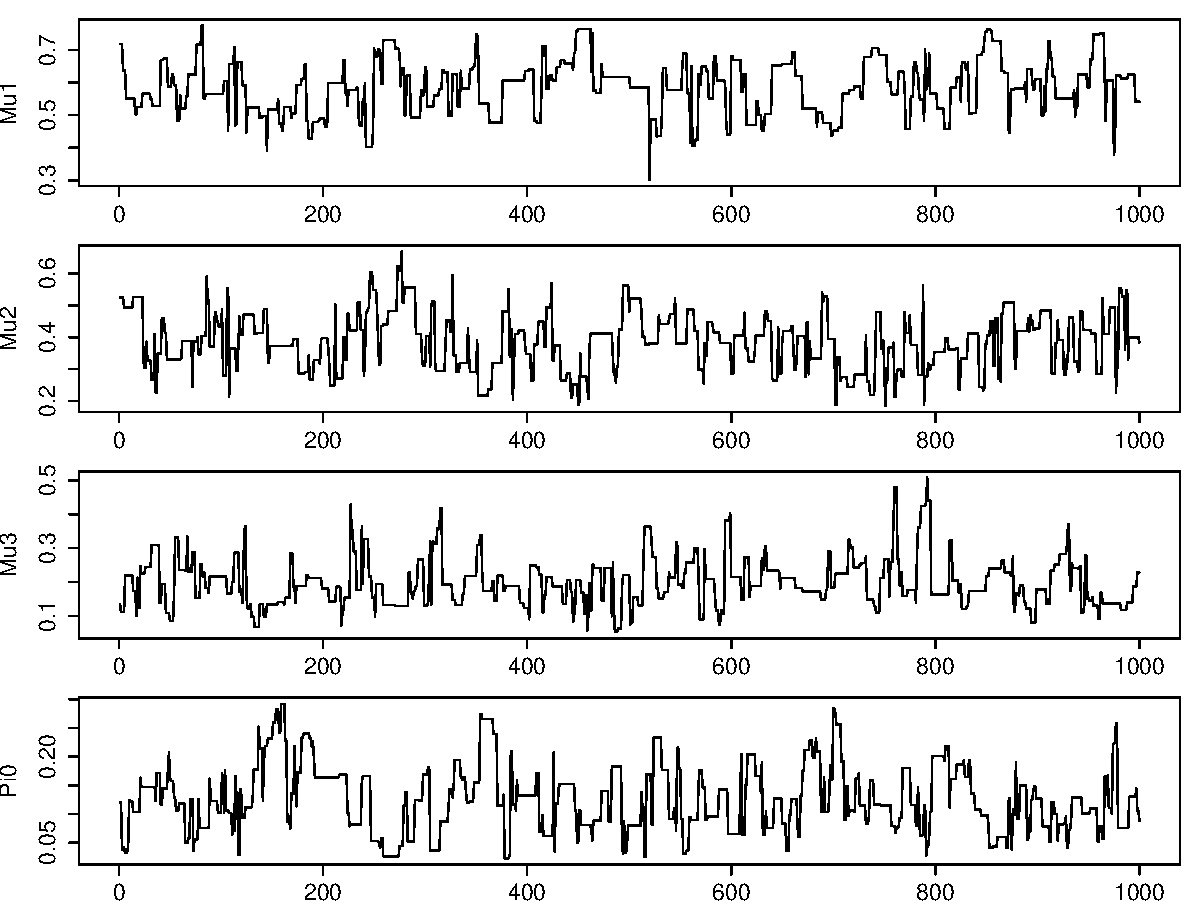
\includegraphics[scale=0.65]{Chains.pdf}
\captionof{figure}{The sampling chains of $(\mu, \pi_0)$}
\end{center}

\begin{center}
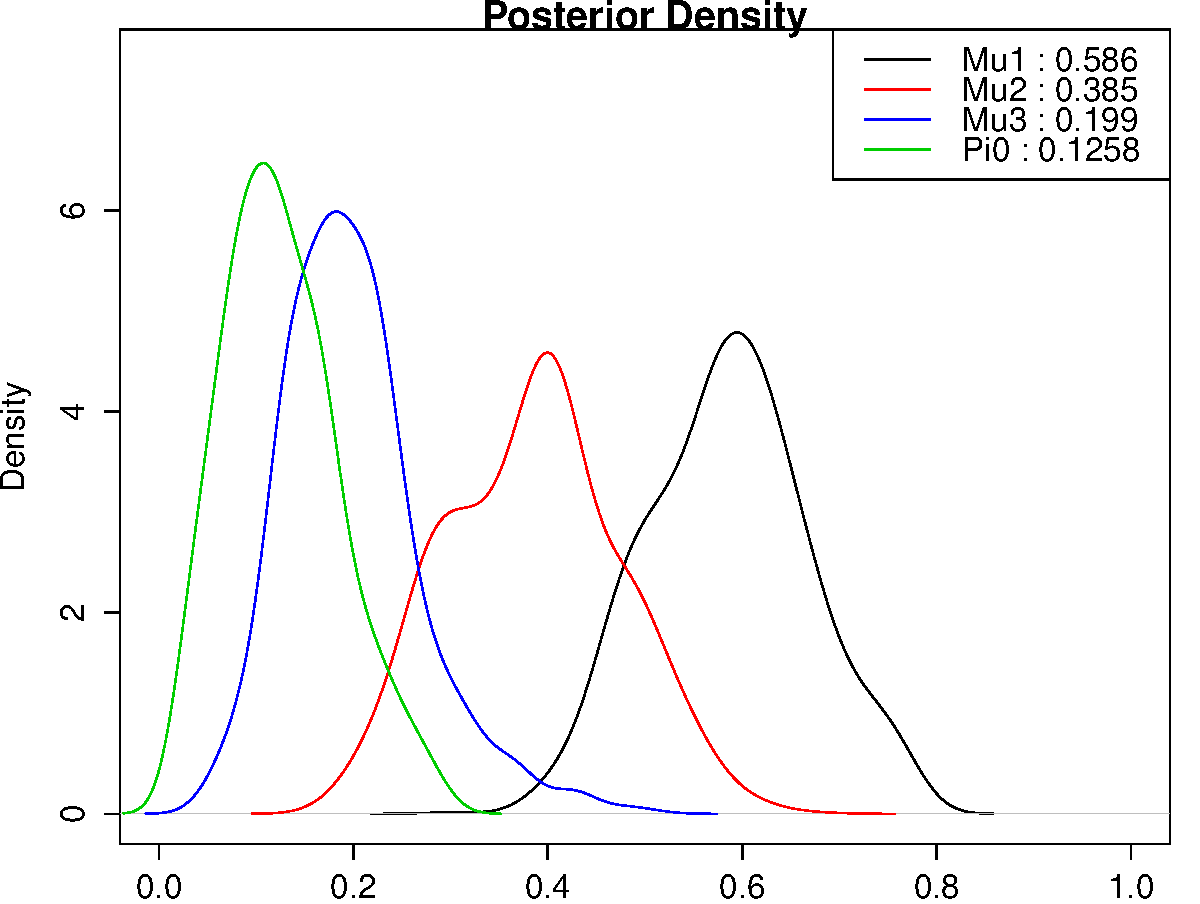
\includegraphics[scale=0.65]{post_k3.pdf}
\captionof{figure}{The Posterior density of $(\mu, \pi_0)$ where the legend shows the posterior mean of each parameter}
\end{center}




%\begin{table}[htbp]
%\begin{adjustwidth}{-0.5in}{-1in}
%\resizebox{0.7\textwidth}{!}{\begin{minipage}{\textwidth}
%\caption{Summary of the model coefficients and standard error estimates}
%\label{tab: coef}
%
%\begin{tabular}{llllll|lllll} 
%\hline 
% \\
%\hline \\
%\end{tabular}
%\end{minipage}}
%\end{adjustwidth}
%\end{table}


\newpage
\section*{Reference}
1. Smith RL . “Efficient Monte-Carlo Procedures for Generating Points Uniformly Dis- tributed over Bounded Regions.” Operations Research, 32(6), 1296–1308 (1984).\\ 
2. Van den Meersche, Karel, K. E. R. Soetaert, and D. J. Van Oevelen. "xsample (): an R function for sampling linear inverse problems." Journal of Statistical Software 30 (2009).


\end{document}






















